\chapter{Plataforma de desarrollo}
\label{cap:capitulo4}

\begin{flushright}
\begin{minipage}[]{10cm}
\emph{Las herramientas adecuadas en las manos adecuadas pueden cambiar el mundo}\\
\end{minipage}\\

Steve Jobs\\
\end{flushright}

\vspace{1cm}

Tras haber establecido los objetivos que se pretenden alcanzar en este proyecto, en este capítulo se van a tratar las distintas plataformas de desarrollo, tanto \textit{hardware} como \textit{software}, que han contribuido a la consecución de dichos objetivos.

\section{Hardware}

En este apartado se van a describir el conjunto de componentes hardware que se han adquirido para llevar a cabo este proyecto. Siguiendo la folosofía \textit{low-cost} y \ac{DIY}, se ha primado el conseguir el menor coste de cada componente.

\subsection{Raspberry Pi 4}

La Raspberry Pi es una computadora de bajo coste y, con su tamaño compacto, es ideal para proyectos de electrónica, programación y educación. Esta placa, en su cuarta versión, dispone de un procesador ARM Cortex-A72 de cuatro núcleos a 1,50GHz fabricado en 28nm, y con tres configuraciones de memoria. Su alimentación la recibe por el puerto USB-C, tiene dos conectores micro HDMI, conexión Wi-Fi, Bluetooh 5.0, dos USB 2.0 y dos USB 3.0. Permite la compatibilidad con la mayoría de accesorios gracias al conector GPIO de cuarenta pines y el conector \ac{CSI}. Gracias a esos cuarenta pines, el usuario puede interactuar con una amplia variedad de dispositivos externos, como sensores, LEDs y motores, lo que la hace excelente para proyectos de automatización y robótica. 

 Sin embargo, la Raspberry Pi usa procesadores ARM, que, aunque eficientes energéticamente, no están optimizados para realizar tareas intensivas de \ac{IA}, como entrenar modelos de redes neuronales o ejecutar inferencias en tiempo real a gran escala. En la Figura \ref{fig:raspberry} se puede ver una imagen de la placa con referencia a las distintas partes de la misma. Esta placa tiene un coste de unos 65€. 


\begin{figure} [h!]
	\begin{center}
		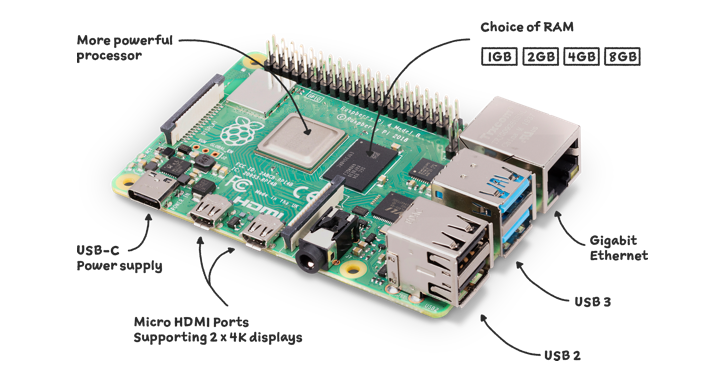
\includegraphics[width=14cm]{figs/raspberrypi4.png}
	\end{center}
	\caption{Raspberry Pi 4$^{\ref{note:enlace38}}$} 
\label{fig:raspberry}
\end{figure}

\setcounter{footnote}{38} % Establecer la numeración de la siguiente nota al pie
\footnotetext[\value{footnote}]{\url{https://www.raspberrypi.com/products/raspberry-pi-4-model-b/}\label{note:enlace38}}

\subsection{Raspberry PiCamera}

Esta cámara (Figura \ref{fig:raspberrycam}) tiene un tamaño de  23.86 x 25 x 9mm, utiliza el sensor de imagen IMX219PQ de Sony, que ofrece imágenes de vídeo de alta velocidad y alta sensibilidad. Dispone también de funciones de control automático, como el control de exposición, el balance de blancos y la detección de luminancia. Para conectarse, usa un cable plano diseñado específicamente para el puerto \ac{CSI} de la placa. Su coste aproximado es de 18€. 

%Es muy importante destacar su bajo coste, lo que le convierte en muy buena opción para hacer aplicaciones \textit{low-cost}. Sin embargo, el cable de la cámara es bastante sensible a tensiones y torsiones y es debido a ello que aunque la cámara fue prestada por la universidad, fue necesario adquirir una unidad más a través de Amazon con un coste aproximado de 18€.    


\begin{figure} [h!]
	\begin{center}
		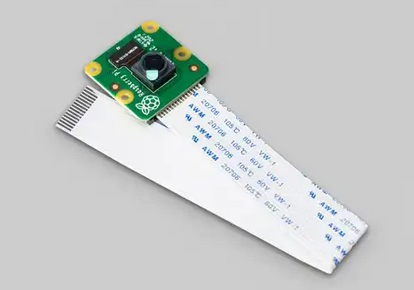
\includegraphics[width=6cm]{figs/campi.png}
	\end{center}
	\caption{Raspberry PiCamera V2$^{\ref{note:enlace39}}$} 
\label{fig:raspberrycam}
\end{figure}

\setcounter{footnote}{39} % Establecer la numeración de la siguiente nota al pie
\footnotetext[\value{footnote}]{\url{https://www.raspberrypi.com/products/camera-module-v2/}\label{note:enlace39}}

\subsection{GPS NEO 6M}

Para poder identificar dónde se encuentra cada bache es necesario hacer uso de un posicionamiento global mediante satélites. En este caso se decidió usar el módulo NEO 6M (Figura \ref{fig:gps}), cuyo precio aproximado es de 9€. Este módulo utiliza el chipset u-blox NEO-6M, que proporciona un seguimiento preciso de la posición utilizando satélites \acs{GPS}, permitiendo determinar la latitud, longitud, altitud, y velocidad. Además, incluye una antena cerámica externa de alta ganancia (puede ser interna en algunas versiones) que mejora la recepción de la señal \acs{GPS}, incluso en áreas con una señal débil.

Tiene una precisión de aproximadamente 2.5 metros en condiciones abiertas. Soporta hasta veintidós satélites simultáneamente, lo que le permite ofrecer posicionamiento confiable y estable. Asimismo, utiliza comunicación por \ac{UART}, comunmente a 9600 bps, lo que facilita su integración con muchas placas del mercado.

\begin{figure} [h!]
	\begin{center}
		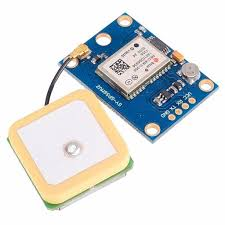
\includegraphics[width=4cm]{figs/GPSNEO6MV2.jpeg}
	\end{center}
	\caption{Módulo GPS NEO 6M$^{\ref{note:enlace40}}$} 
\label{fig:gps}
\end{figure}

\setcounter{footnote}{40} % Establecer la numeración de la siguiente nota al pie
\footnotetext[\value{footnote}]{\url{https://www.u-blox.com/en/product/neo-6-series}\label{note:enlace40}}


\subsection{Sevomotor estándar Parallax}

Este tipo de servo (Figura \ref{fig:parallax}) tiene un rango de rotación de 0 a 180 grados y se puede controlar digitalmente mediante la técnica de \ac{PWM} con un pulso alto de 0.75–2.25 ms en intervalos de 20 ms. Este tipo de servo es muy común en aplicaciones de animatrónica y robótica. Su precio ronda los 17€.
%Sin embargo, su coste ha subido en los últimos años y el precio por unidad ronda los 17€. La universidad ha sido quien me ha prestado estos servomotores pero para esta aplicación no es necesario usarlos y se pueden sustituir por otros de menor precio que cumplan con el requisito de tener rotaciones de 0 a 180 grados (Figura \ref{fig:parallax} derecha), cuyo precio de dos servomotores es de casi 8€. 


%\begin{figure}[ht!]
%	\centering
%	\begin{minipage}{0.2\linewidth}
%		\centering
%		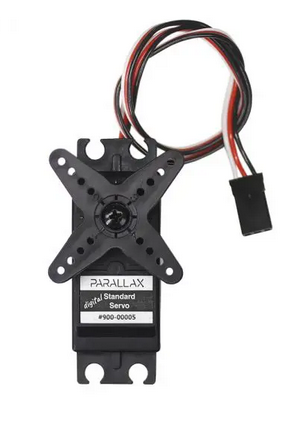
\includegraphics[width=\linewidth]{figs/parallax.png}
%		\caption*{\centering Parallax $^{\ref{note:enlace38}}$} %\cite{memnon_image}
%	\end{minipage}
%	\hspace{2cm}
%	\begin{minipage}{0.33\linewidth}
%		\centering
%		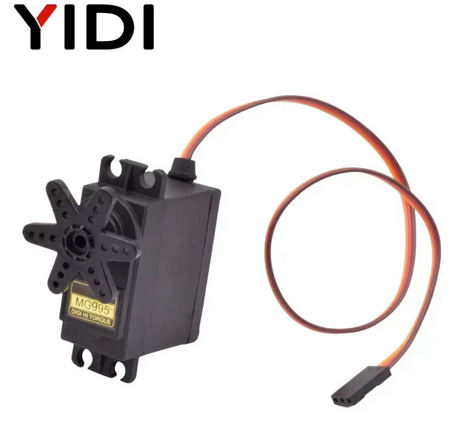
\includegraphics[width=\linewidth]{figs/diyi.png}
%		\caption*{\centering YIDI $^{\ref{note:enlace39}}$} %\cite{gomezguerreros}
%	\end{minipage}
%	\caption{Tipos de Servomotores}
%	\label{fig:parallax}
%\end{figure}

\begin{figure} [h!]
	\begin{center}
		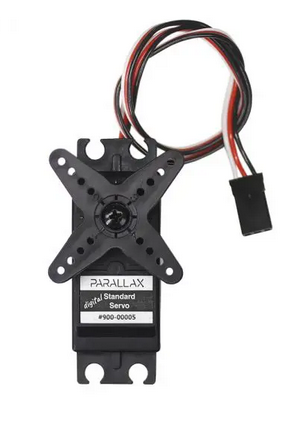
\includegraphics[width=4cm]{figs/parallax.png}
	\end{center}
	\caption{Servomotor Parallax$^{\ref{note:enlace41}}$} 
	\label{fig:parallax}
\end{figure}


\setcounter{footnote}{41} % Reiniciar la numeración de notas al pie
\footnotetext[\value{footnote}]{\url{https://www.parallax.com/product/parallax-standard-servo/}\label{note:enlace41}}

%\setcounter{footnote}{39} % Reiniciar la numeración de notas al pie
%\footnotetext[\value{footnote}]{\url{https://es.aliexpress.com/item/1005004551539283.html?spm=a2g0o.productlist.main.15.bee4rd8Srd8SSO&algo_pvid}\label{note:enlace39}}

\subsection{Ruedas}

Para implementar las ruedas del prototipo robótico de este proyecto se decidió tomar las ruedas del kit robótico ActivityBot, que usa unas ruedas compatibles con los motores descritos anteriormente, además de ser muy ligeras y estables. Se trata de una rueda de plástico con neumático tipo junta tórica (Figura \ref{fig:wheel} izquierda). El perfil estrecho convierte a esta rueda en ideal para aplicaciones que requieren una dirección precisa, y el diámetro de la rueda es de 66mm. También se pueden adquirir individualmente, con un coste de 4,54€ la unidad.

Para enriquecer el proyecto, se han empleado otro tipo de ruedas cuyo diámetro es igual a las ruedas del ActivityBot pero el grosor del neumático es superior y tiene un mayor agarre sobre la superficie. En este caso son ruedas con el neumático azul (Figura \ref{fig:wheel} derecha) pero existen de muchos tipos y con precio similar a las ruedas ActivityBot.

\begin{figure}[ht!]
	\centering
	\begin{minipage}{0.4\linewidth}
			\centering
			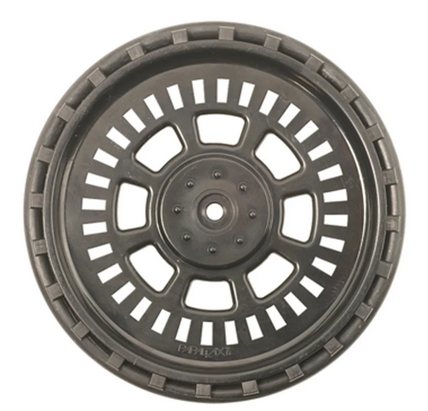
\includegraphics[width=\linewidth]{figs/wheel.png}
			\caption*{\centering Rueda ActivityBot $^{\ref{note:enlace42}}$} 
		\end{minipage}
	\hspace{2cm}
	\begin{minipage}{0.38\linewidth}
			\centering
			\includegraphics[width=\linewidth]{figs/wheel2.png}
			\caption*{\centering Rueda Azul genérica $^{\ref{note:enlace43}}$} 
		\end{minipage}
	\caption{Ruedas utilizadas}
	\label{fig:wheel}
\end{figure}


\setcounter{footnote}{42} % Establecer la numeración de la siguiente nota al pie
\footnotetext[\value{footnote}]{\url{https://es.rs-online.com/web/p/accesorios-para-kits-de-desarrollo/8430897?srsltid=AfmBOorv3a6_tQNdqAoKx_21Mn1m2MAum68oApyvr5mq8ExPTuh_CVNy}\label{note:enlace42}}

\setcounter{footnote}{43} % Establecer la numeración de la siguiente nota al pie
\footnotetext[\value{footnote}]{\url{https://es.aliexpress.com/item/1005005145020093.html}\label{note:enlace43}}


\subsection{Google Coral USB}

El Google Coral USB Accelerator (Figura \ref{fig:googlecoral}) es un dispositivo que permite acelerar tareas de \ac{IA} en dispositivos que no cuentan con hardware especializado para ello. Está diseñado para ejecutarse con modelos de aprendizaje automático utilizando la unidad de procesamiento de tensores de Google, lo que mejora significativamente la velocidad de inferencia en aplicaciones de \acs{IA}. Está optimizado para ejecutar modelos preentrenados en TensorFlow Lite, la versión ligera de TensorFlow diseñado para dispositivos con recursos limitados. Al ser una placa lanzada hace varios años al mercado, sólo es compatible con  las versiones de Python 3.6 hasta la 3.9.

Por sus cualidadesdescritas, se ha decidido este componente para mejorar la detección de baches en tiempo real y solventar las limitaciones de la Raspberry Pi. Su precio es de unos 65€.
 
\begin{figure} [h!]
	\begin{center}
		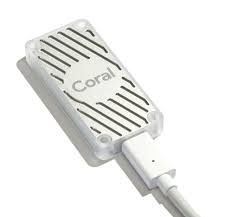
\includegraphics[width=4cm]{figs/googlecoral.png}
	\end{center}
	\caption{Google Coral USB$^{\ref{note:enlace44}}$} 
	\label{fig:googlecoral}
\end{figure}

\setcounter{footnote}{44} % Establecer la numeración de la siguiente nota al pie
\footnotetext[\value{footnote}]{\url{https://coral.ai/products/accelerator/}\label{note:enlace44}}

\subsection{Power bank}

Para poder alimentar a todos los componentes se ha incluido en el prototipo robótico una \textit{power bank} de gran capacidad para que permita la autonomía del robot durante un tiempo más que razonable. Concretamente, se ha elegido la Xiaomi Redmi Power Bank de 20000 mAh, cuyas dimensiones son: 73,6 x 27,3 x 154 mm y después de muchos ciclos de carga y descarga, mantienen un buen rendimiento sin perder demasiada capacidad. Su precio ronda los 20€. % peso de 400g

\begin{figure} [h!]
	\begin{center}
		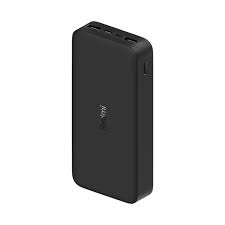
\includegraphics[width=5cm]{figs/powerbank.png}
	\end{center}
	\caption{Xiaomi Power bank$^{\ref{note:enlace45}}$} 
	\label{fig:powerbank}
\end{figure}

\setcounter{footnote}{45} % Establecer la numeración de la siguiente nota al pie
\footnotetext[\value{footnote}]{\url{https://ams.buy.mi.com/es/item/3202200053?&skupanel=1}\label{note:enlace45}}

\subsection{Rueda loca}

Para poder conseguir un movimiento correcto y poder encontrar el punto de apoyo para el robot, es necesario incorporar al robot una rueda loca. Tras investigar qué rueda encajaba mejor, se ha decidido incluir una rueda loca como la que aparece en la Figura \ref{fig:ruedaloca}, que tiene las siguientes dimensiones: 5,3 x 2,9 x 2 cm. El precio de esta es de 1,13€.

\begin{figure} [h!]
	\begin{center}
		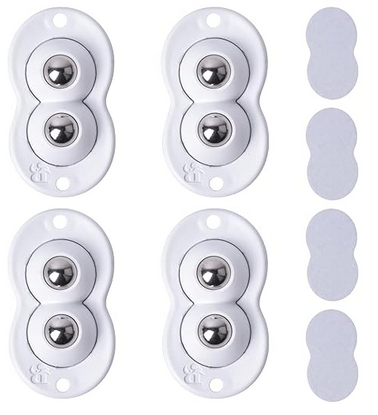
\includegraphics[width=4cm]{figs/ruedaloca.png}
	\end{center}
	\caption{Rueda loca$^{\ref{note:enlace46}}$} 
	\label{fig:ruedaloca}
\end{figure}

\setcounter{footnote}{46} % Establecer la numeración de la siguiente nota al pie
\footnotetext[\value{footnote}]{\url{https://www.amazon.es/dp/B0BZZCJJT8?ref=cm_sw_r_mwn_dp_N64JV6SGENWN4YPSD849&ref_=cm_sw_r_mwn_dp_N64JV6SGENWN4YPSD849&social_share=cm_sw_r_mwn_dp_N64JV6SGENWN4YPSD849&language=es-ES}\label{note:enlace46}}

\subsection{Ordenador principal}

Para poder desarrollar programas, hacer pruebas en simulación, permitir conectarse por SSH a la Raspberry Pi y poder comandar acciones al robot, ha sido necesario tener un ordenador principal que permitiera realizar todas las tareas. El ordenador que aparece en la Figura \ref{fig:ordenador} es el que se ha empleado en este proyecto, y cumple las características descritas en el Cuadro \ref{cuadro:carac_ordena}.


\begin{figure} [h!]
	\begin{center}
		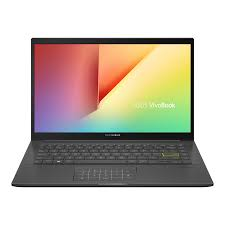
\includegraphics[width=4cm]{figs/ordenador.png}
	\end{center}
	\caption{ASUS VivoBook 14$^{\ref{note:enlace47}}$} 
	\label{fig:ordenador}
\end{figure}

\setcounter{footnote}{47} % Establecer la numeración de la siguiente nota al pie
\footnotetext[\value{footnote}]{\url{https://www.asus.com/es/laptops/for-home/vivobook/vivobook-14-k413/}\label{note:enlace47}}

\begin{table}[H]
	\begin{center}
		\begin{tabular}{|c|c|}
			\hline
			\textbf{Características} & \textbf{Descripción} \\
			\hline
			\multirow{4}{*}{Pantalla} & \multirow{4}{*}{\shortstack{ 14 pulgadas \\ Full HD (1920x1080) \\ tecnología LED \\antirreflejo }}\\
			& \\
			& \\
			& \\
			\hline
			Procesador (CPU) & Intel Core i7 de 10ª generación \\
			\hline
			Memoria RAM & 8GB \\
			\hline
			Almacenamiento & 512GB \\
			\hline
			Tarjeta gráfica (GPU) & Intel UHD Graphics de Comet Lake-U GT2 \\
			\hline
			Sistema Operativo & Windows 10 y Ubuntu 22.04 \\
			\hline
			\multirow{6}{*}{Puertos} &\multirow{6}{*}{\shortstack{1x USB 3.2 Gen 1 Tipo-A \\1x USB 3.2 Gen 1 Tipo-C \\ 2x USB 2.0 \\ 1x HDMI \\lector de tarjetas microSD \\entrada combo de audio }}\\  
			& \\
			& \\
			& \\
			& \\
			& \\
			\hline
			Conectividad & 	Wi-Fi 5 (802.11ac), Bluetooth 4.1 / 5.0 \\
			\hline
			Batería & 37 Whr \\
			\hline
			Peso & 1.4 kg \\
			\hline
			Dimensiones & 32.5 x 21.6 x 1.99 cm \\
			\hline
		\end{tabular}
		\caption{Especificaciones técnicas del ordenador usado}
		\label{cuadro:carac_ordena}
	\end{center}
\end{table}


\section{Software}

En este apartado se van a describir los programas y librerías que han sido necesarios usar cumplir con los objetivos descritos en el Capítulo 3.

\subsection{Ubuntu}

Ubuntu\footnote{\url{https://ubuntu.com/}} (Figura \ref{fig:ubuntu}) es una de las muchas distribuciones del sistema operativo GNU/Linux; esta, concretamente, está basada en Debian GNU/Linux, y es mantenida por Canonical Ltd. Puede utilizarse en ordenadores y servidores. Está orientado al usuario promedio, con un fuerte enfoque en la facilidad de uso y en mejorar la experiencia del usuario; es por ello que se ha convertido en uno de los sistemas operativos más populares, cuenta con una amplia comunidad de soporte que le brinda continuamente actualizaciones, que incluyen parches de seguridad y mejoras.

\begin{figure} [h!]
	\begin{center}
		
\includegraphics[width=4cm]{figs/ubuntu.png}
	\end{center}
	\caption{Logo de Ubuntu} %$^{\ref{note:enlace51}}$
	\label{fig:ubuntu}
\end{figure}

%\setcounter{footnote}{51} % Establecer la numeración de la siguiente nota al pie
%\footnotetext[\value{footnote}]{\url{https://ubuntu.com/}\label{note:enlace51}}

Entre todas las versiones existentes de Ubuntu, para la realización del proyecto se ha usado Ubuntu 22.04 LTS y Ubuntu 20.04 LTS. El ordenador usado (descrito en el Apartado 4.1.9) tiene instalado Ubuntu 22.04 \ac{LTS} pero el robot inicialmente usaba Ubuntu 22.04 y finalmente está usando Ubuntu 20.04 \acs{LTS} Server, una versión de Ubuntu sin interfaz gráfica. La decisión de usar Ubuntu 20.04 es debido a que el dispositivo Google Coral USB (descrito en el Apartado 4.1.6) es compatible con versiones de Python entre 3.6 y 3.9, y en Ubuntu 22.04 la versión de Python que se instala por defecto es la 3.10, y el intento de cambiar dicha versión genera numerosos problemas de dependencias, sobre todo con la versión de ROS 2 usada. Asimismo, en numerosos foros aconsejaban migrar a Ubuntu 20.04\footnote{\url{https://robotics.stackexchange.com/questions/104413/}} que usa Python 3.8. En el Cuadro \ref{cuadro:ubuntu} se muestran algunas de las diferencias entre Ubuntu 22.04 y Ubuntu 20.04.

\begin{table}[H]
	\begin{center}
		\begin{tabular}{|c|c|c|}
			\hline
			\textbf{Características} & \textbf{Ubuntu 20.04} & \textbf{Ubuntu 22.04} \\
			\hline
			Fecha de lanzamiento & Abril 2020 & Abril 2022\\
			\hline
			Soporte & Hasta Abril 2025 & Hasta Abril 2027\\
			\hline
			Kernel & Linux 5.4 & Linux 5.15 \\
			\hline
			Entorno de escritorio & GNOME 3.36 & GNOME 42\\
			\hline
			Python & Python 3.8 & Python 3.10\\
			\hline
			Soporte gráfico NVIDIA & Soporte estándar & Soporte mejorado con Wayland\\
			\hline
		\end{tabular}
		\caption{Diferencias entre Ubuntu 20.04 y Ubuntu 22.04}
		\label{cuadro:ubuntu}
	\end{center}
\end{table}

\subsection{FreeCAD}

Esta herramienta de código abierto\footnote{\url{https://www.freecad.org/}} (Figura \ref{fig:freecad}) es un \textit{software} de diseño asistido por ordenador utilizado principalmente para la creación de modelos 3D en diferentes áreas, como la ingeniería, arquitectura, y diseño de productos. Está diseñado para ser altamente modular, formado por \textit{workbenches}, lo que permite a los usuarios adaptar y extender su funcionalidad según sus necesidades.

FreeCAD se basa en el concepto de modelado paramétrico, lo que permite modificar el diseño fácilmente. Los usuarios pueden retroceder en la historia de un modelo y cambiar parámetros que actualizan automáticamente el diseño. También FreeCAD es multiplataforma, cuenta con una consola de Python integrada y soporta una amplia gama de formatos de archivo como STL y SVG, entre otros. Esta ha sido la herramienta elegida para hacer el diseño 3D de la pieza y la generación del formato STL para su posterior impresión. 

\begin{figure} [h!]
	\begin{center}
		
\includegraphics[width=3cm]{figs/freecad.png}
	\end{center}
	\caption{Logo de Freecad} % $^{\ref{note:enlace48}}$
	\label{fig:freecad}
\end{figure}

%\setcounter{footnote}{48} % Establecer la numeración de la siguiente nota al pie
%\footnotetext[\value{footnote}]{\url{https://www.freecad.org/}\label{note:enlace48}}

\subsection{Python}

Python\footnote{\url{https://es.python.org/}} (Figura \ref{fig:python}) es un lenguaje de programación de alto nivel, interpretado y de propósito general, ampliamente reconocido por su simplicidad y legibilidad. Fue creado por Guido van Rossum y lanzado por primera vez en 1991, y ha crecido rápidamente en popularidad debido a su versatilidad y facilidad de uso, tanto para principiantes como para programadores experimentados, lo que le convierte en un lenguaje multiplataforma y multiparadigma.

Python es un lenguaje interpretado, lo que significa que el código se ejecuta línea a línea sin necesidad de ser compilado. Esto facilita el desarrollo rápido y la depuración. Tiene una sintaxis sencilla, legible y es ampliamente utilizado en áreas como: desarrollo web (Django y Flask), ciencia de datos y aprendizaje automático (NumPy, Pandas, TensorFlow, y PyTorch), automatización y scripting, entre otros.

Debido a esa simplicidad y versatilidad, en Raspberry Pi se considera Python como uno de los lenguajes de programación oficiales recomendados, y es por ello que se ha decidido usar este lenguaje para este proyecto.

\begin{figure} [h!]
	\begin{center}
		
\includegraphics[width=4cm]{figs/python.png}
	\end{center}
	\caption{Logo de Python}  % $^{\ref{note:enlace49}}$
	\label{fig:python}
\end{figure}

%\setcounter{footnote}{49} % Establecer la numeración de la siguiente nota al pie
%\footnotetext[\value{footnote}]{\url{https://es.python.org/}\label{note:enlace49}}

\subsubsection{Software matemático}

NumPy (Numerical Python) es una biblioteca fundamental para el cálculo numérico en Python. Está diseñada para facilitar el manejo eficiente de vectores, grandes matrices y arrays multidimensionales, junto con una amplia colección de funciones matemáticas para realizar operaciones sobre estos arrays. Se ha usado en este proyecto para poder calcular el área del bache.

\subsubsection{Software para localización}

PyNMEA2 es una biblioteca de Python que se utiliza para analizar y generar mensajes en formato NMEA (National Marine Electronics Association) (Figura \ref{fig:nmea}), un estándar utilizado en dispositivos GPS y otros sistemas de navegación marina. Es especialmente útil cuando trabajas con módulos GPS en proyectos de Raspberry Pi u otros dispositivos embebidos, ya que te permite interpretar la información que estos dispositivos envían, como la localización, velocidad y tiempo.

\begin{figure} [h!]
	\begin{center}
		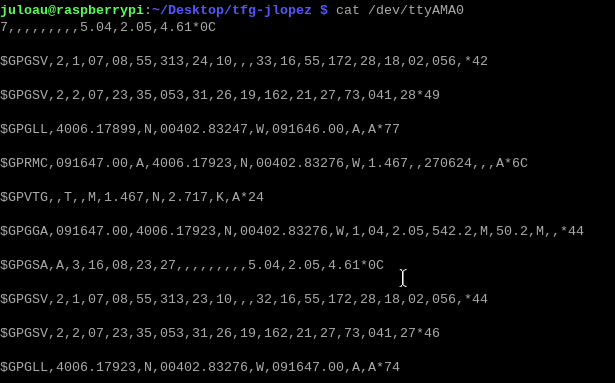
\includegraphics[width=12cm]{figs/workinggps.png}
	\end{center}
	\caption{Sentencias NMEA capturadas del GPS} %$^{\ref{note:enlace50}}$
	\label{fig:nmea}
\end{figure}

PyNMEA2 te permite interpretar las sentencias NMEA, que son los datos en bruto que los módulos GPS envían, usualmente en forma de texto. Algunas sentencias comunes son:

\$GPGGA: proporciona datos como la latitud, longitud, y altitud.

\$GPRMC: contiene información esencial de ubicación, velocidad y tiempo.

\$GPGLL: latitud y longitud.

Es este proyecto, se van a emplear las sentencias que contengan latitud y longitud para estimar la ubicación de cada bache.

\subsection{OpenCV}

OpenCV\footnote{\url{https://opencv.org/}} (Figura \ref{fig:opencv}) es una biblioteca software de código abierto diseñada para la visión artificial y el procesamiento de imágenes. Fue desarrollada inicialmente por Intel en 1999 y ahora es mantenida por una gran comunidad de desarrolladores. OpenCV es ampliamente utilizada en aplicaciones que requieren análisis de imágenes, detección de objetos, reconocimiento de rostros, visión computacional, y mucho más. En este proyecto se ha usado concretamente para la detección del bache y el cálculo del área.

\begin{figure} [h!]
	\begin{center}
		
\includegraphics[width=3cm]{figs/opencv.png}
	\end{center}
	\caption{Logo de OpenCV} %$^{\ref{note:enlace50}}$
	\label{fig:opencv}
\end{figure}

%\setcounter{footnote}{50} % Establecer la numeración de la siguiente nota al pie
%\footnotetext[\value{footnote}]{\url{https://opencv.org/}\label{note:enlace50}}

\subsection{ROS 2}

ROS, por sus siglas en inglés, \textit{Robot Operating System} se trata de un conjunto de bibliotecas y herramientas que ayudan a los desarrolladores a construir sistemas robóticos. ROS proporciona servicios de nivel bajo como abstracción de hardware, control de dispositivos, paso de mensajes entre procesos y gestión de paquetes, así como herramientas para simulación, pruebas y desarrollo de algoritmos.

ROS 2, la segunda generación de ROS, se ha rediseñado para superar las limitaciones de su predecesor. Está basado en un nuevo middleware llamado DDS (Data Distribution Service), que permite una mejor comunicación entre nodos, mayor seguridad, y más opciones de transporte y calidad de servicio (QoS). También mejora la escalabilidad, el soporte para sistemas distribuidos y la capacidad para aplicaciones en tiempo real. Además, ROS 2 es multiplataforma e interoperable; soportando múltiples lenguajes de programación, como C++ y Python.

%de un \textit{middleware} para programar robots. Un \textit{middleware} es una capa de software entre el sistema operativo y las aplicaciones de usuario que permiten llevar a cabo aplicaciones \textit{software} independiente del dominio que ese encuentre. Es decir, ROS aporta un conjunto de herramientas, bibliotecas y convenciones. También, ofrecen desarrollo, integración, ejecución y herramienta de monitorización. El número 2 indica que es la segunda generación de este middleware. 

%ROS 2 tiene tres diferentes dimensiones: la comunidad de ROS 2 que contribuye al desarrollo de aplicaciones es enorme, el grafo de computación de una aplicación en ROS 2 está formado por nodos conectados con distintos paradigmas de comunicación y el espacio de trabajo, también conocido como \textit{workspace}, es aquel que se trata del \textit{software} instalado que se divide a su vez en \textit{underlay} (la instalación básica de ROS 2) y \textit{overlay} (son el resto de programas que se desarrollan).

Según se ha explicado en el Apartado 4.2.4, debido a que se ha necesitado para este proyecto usar Ubuntu 20.04 y Ubuntu 22.04; se ha tenido que usar las dos distribuciones más estable de ROS para cada versión de Ubuntu: ROS 2 Foxy\footnote{\url{https://docs.ros.org/en/foxy/Installation.html}} y ROS 2 Humble\footnote{\url{https://docs.ros.org/en/humble/index.html}}, respectivamente (Figura \ref{fig:rosdis}).


\begin{figure}[ht!]
	\centering
	\begin{minipage}{0.35\linewidth}
		\centering
		
\includegraphics[width=\linewidth]{figs/foxy.png}
		\caption*{\centering Logo ROS 2 Foxy} % $^{\ref{note:enlace54}}$
	\end{minipage}
	\hspace{2cm}
	% aquí incluir iamgen de Guerrero de terracota
	\begin{minipage}{0.35\linewidth}
		\centering
		
\includegraphics[width=\linewidth]{figs/humble.png}
		\caption*{\centering Logo ROS 2 Humble} % $^{\ref{note:enlace55}}$
	\end{minipage}
	\caption{Distribuciones de ROS 2 usadas}
	\label{fig:rosdis}
\end{figure}


%\setcounter{footnote}{54} % Reiniciar la numeración de notas al pie
%\footnotetext[\value{footnote}]{\url{https://docs.ros.org/en/foxy/Installation.html}\label{note:enlace54}}

%\setcounter{footnote}{55} % Reiniciar la numeración de notas al pie
%\footnotetext[\value{footnote}]{\url{https://docs.ros.org/en/humble/index.html}\label{note:enlace55}}


\subsubsection{ROS 2 Control}
ROS 2 Control\footnote{\url{https://control.ros.org/rolling/doc/getting_started/getting_started.html}} es un framework dentro de ROS 2 diseñado para facilitar el control de robots en tiempo real. Proporciona una infraestructura modular y escalable para manejar controladores que gestionan los actuadores (motores, servomotores, etc.) de un robot, así como la lectura de sensores. Se utiliza comúnmente en robots móviles, brazos robóticos, drones y otras plataformas robóticas.

Los componentes principales de ROS 2 Control son:

\begin{itemize}
	%\item \textit{User interface}. Pueden interactuar con el sistema mediante servicios y una interfaz de línea de comandos.
	\item \textit{Hardware Components/Interfaces}. Realizan comunicación con \textit{hardware} físico y pueden ser: sistemas, sensores y actuadores. Cada \textit{hardware} tendrá una serie de \textit{command interfaces} o de \textit{state interfaces} que permitirán monitorizar o interactuar con cada componente.
	\item \textit{Resource Manager}. Abstrae y gestiona los \textit{hardware interfaces}, permitiendo la abstracción de los \textit{state interfaces} y los \textit{command interfaces}.
	\item\textit{Controller Manager}. Gestiona controladores e interfaces de hardware en el framework ROS 2 Control.
	\item \textit{Controllers}. Utilizan la teoría de control para interactuar con el hardware. Pueden ser creados desde cero o usar los que viene por defecto de la librería de ROS 2 Control, que suplen las necesidades en la mayoría de las ocasiones.
\end{itemize}

En este proyecto se ha decidido usar ROS 2 Control para crear un modelo del robot en simulación y poder trabajar con él usando la filosofía de ROS 2 Control.


\subsection{Gazebo}

Gazebo\footnote{\url{https://gazebosim.org/home}} (Figura \ref{fig:gazebo}) es un simulador de robots que permite modelar entornos físicos tridimensionales y probar robots en ellos sin necesidad de tener el robot físico y evitar así posibles caídas o golpes. Es ampliamente utilizado en la investigación y desarrollo de robótica, especialmente en combinación con ROS y ROS 2. Además, ofrece una simulación realista en un entorno 3D, y por ello se decidió usar este simulador para el proyecto.

\begin{figure} [h!]
	\begin{center}
		
\includegraphics[width=4cm]{figs/gazebo.png}
	\end{center}
	\caption{Logo de Gazebo} % $^{\ref{note:enlace57}}$
	\label{fig:gazebo}
\end{figure}

%\setcounter{footnote}{57} % Establecer la numeración de la siguiente nota al pie
%\footnotetext[\value{footnote}]{\url{https://gazebosim.org/home}\label{note:enlace57}}

\subsection{Herramientas de monitorización}

Para el desarrollo del proyecto, se emplean diversas herramientas de monitorización que permiten visualizar y controlar los datos y procesos dentro del entorno de ROS 2, y para ello se ha decidido usar las herramientas que se describen a continuación.

\subsubsection{Rviz}

RViz\footnote{\url{http://wiki.ros.org/rviz}} (Figura \ref{fig:rviz}) es una herramienta de visualización en 3D utilizada en ROS y ROS 2 para representar información del sistema robótico. Permite a los usuarios ver, en tiempo real, datos como la posición de un robot, sensores, cámaras, mapas y otros elementos. Se ha utilizado para monitorear el comportamiento del robot en simulación.\\

\begin{figure} [h!]
	\begin{center}
		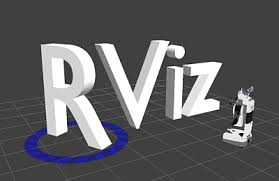
\includegraphics[width=4cm]{figs/rviz.png}
	\end{center}
	\caption{Logo de Rviz} %$^{\ref{note:enlace58}}$
	\label{fig:rviz}
\end{figure}

%\setcounter{footnote}{58} % Establecer la numeración de la siguiente nota al pie
%\footnotetext[\value{footnote}]{\url{http://wiki.ros.org/rviz}\label{note:enlace58}}

\subsubsection{RQT Image View}

RQt Image View\footnote{\url{http://wiki.ros.org/rqt_image_view}} es una herramienta gráfica dentro del ecosistema de ROS y ROS 2 que permite visualizar imágenes en tiempo real de un flujo de datos de imágenes publicado por una cámara en un sistema robótico. Se ha usado esta herramienta para monitorizar la cámara del robot físico.

\subsubsection{ROS2cli}

ROS 2 \ac{CLI}\footnote{\url{https://docs.ros.org/en/humble/Tutorials/Beginner-CLI-Tools.html}} es una herramienta que permite interactuar con el sistema ROS 2 mediante comandos desde la terminal. Ofrece una forma rápida y sencilla de acceder a las funciones y características de ROS 2 sin necesidad de escribir o ejecutar código complejo. Ha sido la herramienta principal en este proyecto para ejecutar los distintos nodos, comprobar si estaban bien lanzados, si se producía buena comunicación entre ellos, entre otras aplicaciones.


\subsection{Google Colaboratory}

Google Colaboratory\footnote{\url{https://colab.research.google.com/}} (Figura \ref{fig:googlecolab}) es un servicio en la nube proporcionado por Google que permite escribir y ejecutar código en Python a través de un entorno de Jupyter Notebook. No requiere configuración para su uso y proporciona acceso gratuito a recursos de computación, incluidos GPUs y TPUs. Es especialmente usado para el aprendizaje automático, la ciencia de datos y la educación. Gracias a esta herramienta, se puede cumplir el requisito nº.4 de los indicados en la sección 3.2.

\begin{figure} [h!]
	\begin{center}
		
\includegraphics[width=4cm]{figs/googlecolab.png}
	\end{center}
	\caption{Logo de Google Colab} %$^{\ref{note:enlace61}}$
	\label{fig:googlecolab}
\end{figure}

%\setcounter{footnote}{61} % Establecer la numeración de la siguiente nota al pie
%\footnotetext[\value{footnote}]{\url{https://colab.research.google.com/}\label{note:enlace61}}

\subsection{YOLOv8}

\acs{YOLO}v8\footnote{\url{https://docs.ultralytics.com/es}} (Figura \ref{fig:yolov8}) desarrollado por la empresa Ultralytics, es una versión avanzada del popular modelo de detección de objetos \ac{YOLO}, diseñado para identificar y localizar objetos en imágenes y videos en tiempo real. Esta versión es conocida por su eficiencia y precisión en la detección de objetos. Es compatible con TensorFlow y PyTorch. También ofrece optimización para diferentes plataformas, incluidos como EdgeTPU, para dispositivos con recursos limitados como puede ser Raspberry Pi. Por todo lo anterior, esta herramienta ha sido elegida para el entrenamiento del modelo de detección de baches. 

\begin{figure} [h!]
	\begin{center}
		
\includegraphics[width=4cm]{figs/yolov8.png}
	\end{center}
	\caption{Logo de YOLOv8} % $^{\ref{note:enlace62}}$
	\label{fig:yolov8}
\end{figure}

%\setcounter{footnote}{62} % Establecer la numeración de la siguiente nota al pie
%\footnotetext[\value{footnote}]{\url{https://docs.ultralytics.com/es}\label{note:enlace62}}

\subsection{TensorFlow Lite}

TensorFlow es una plataforma de código abierto desarrollada por Google para el aprendizaje automático y el desarrollo de redes neuronales. Su diseño permite a los desarrolladores e investigadores crear, entrenar y desplegar modelos de aprendizaje automático de manera eficiente en una variedad de dispositivos, desde ordenadores de alto rendimiento hasta dispositivos con recursos limitados como puede ser Raspberry Pi. Concretamente, para poder ejecutar modelos en dispositivos como las Raspberry Pi,se usa la versión TensorFlow Lite\footnote{\url{https://ai.google.dev/edge/litert}} (Figura \ref{fig:tflite}), ya que está preparada para optimizar los modelos. Es por ello que cualquier modelo que se quiera usar se tiene que convertir a este formato. 

\begin{figure} [h!]
	\begin{center}
		
\includegraphics[width=6cm]{figs/tflite.png}
	\end{center}
	\caption{Logo de TensorFlow Lite} % $^{\ref{note:enlace63}}$ 
	\label{fig:tflite}
\end{figure}

%\setcounter{footnote}{63} % Establecer la numeración de la siguiente nota al pie
%\footnotetext[\value{footnote}]{\url{https://ai.google.dev/edge/litert}\label{note:enlace63}}

\subsection{Interfaz Web}

Para poder hacer más amigable la interacción humano-robot, se ha decidido plasmar los datos obtenidos a través de una interfaz web, y para ello se ha decidido usar las herramientas que se describen a continuación.
 
\subsubsection{ROS2bridge Server}

ROS2bridge Server\footnote{\url{http://wiki.ros.org/rosbridge_server}} es parte de ros2bridge\_suite, y ofrece una capa de transporte WebSocket para la comunicación bidireccional entre páginas web y ROS 2. Convierte mensajes JSON en llamadas a ROS 2 y viceversa, permitiendo que las páginas web interactúen con ROS 2. 

\subsubsection{OpenStreetMaps}

OpenStreetMaps\footnote{\url{https://www.openstreetmap.org}} (Figura \ref{fig:osm}) es un proyecto internacional colaborativo desde 2004 que proporciona datos geográficos gratuitos y abiertos, permitiendo la creación de mapas detallados y editables de cualquier parte del mundo por usuarios voluntarios que den crédito a OpenStreetMaps. Esta herramienta es utilizada en una amplia gama de aplicaciones, incluyendo navegación, análisis de datos geográficos, y proyectos de código abierto relacionados con mapas y geolocalización.


\begin{figure} [h!]
	\begin{center}
		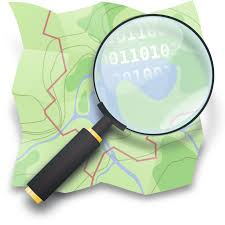
\includegraphics[width=4cm]{figs/osm.png}
	\end{center}
	\caption{Logo de Open Street Maps}  %$^{\ref{note:enlace65}}$
	\label{fig:osm}
\end{figure}\ 

%\setcounter{footnote}{65} % Establecer la numeración de la siguiente nota al pie
%\footnotetext[\value{footnote}]{\url{https://www.openstreetmap.org}\label{note:enlace65}}



Tras conocer todas las plataformas software y hardware empleadas para la realización del presente trabajo fin de grado, es el momento de describir el desarrollo completo llevado a cabo para la construcción hardware del robot  y su correspondiente soporte software, lo que se explicará detalladamente en los siguientes capítulos.
